
\begin{table*}[t!]
  \centering
  \begin{minipage}[t][11.8cm][t]{0.505\linewidth}
    \centering
    \captionsetup{justification=centering}    
    \begin{minted}[xleftmargin=1em,linenos,autogobble,tabsize=2,framesep=1pt,frame=single,fontfamily=courier,fontsize=\fontsize{8}{9}\selectfont]{scala}
			import DFiant._
			
			trait MA4 extends DFDesign {
				val a    = DFSInt[16] <> IN init 0
				val b    = DFSInt[16] <> IN init 0
				val c    = DFSInt[16] <> IN init 0
				val d    = DFSInt[16] <> IN init 0
				val o    = DFSInt[16] <> OUT
				
				def ma(src : DFSInt[16]) = {     
					val acc = DFSInt[18] init 0    //-Compiled to->
					acc := acc - src.prev(4) + src //-Compiled to->
					(acc / 4).toWidth(16)
				}
				def avg2(src1 : DFSInt[16], src2 : DFSInt[16]) =
					((src1 + src2).wc / 2).toWidth(16)
					//  (_ + _).wc is a with-carry addition
					
				o := avg2(
					avg2(ma(a), ma(b)), avg2(ma(c), ma(d))
				)
			}
			
			
			
			
			
			
			
			
			
			object MA4App extends DFApp.VHDLCompiler[MA4]
    \end{minted}
    \captionof{figure}{The MA4 DFiant code \\ Concise and portable}
    \label{fig:MADFiant}
  \end{minipage}
  \hfill
  \begin{minipage}[t][11.8cm][t]{0.49\linewidth}
    \centering
    \captionsetup{justification=centering}
		\begin{minted}[xleftmargin=1em,autogobble,tabsize=2,framesep=1pt,frame=single,fontfamily=courier,fontsize=\fontsize{8}{9}\selectfont]{vhdl}
			...
			signal acc       : signed(17 downto 0);
			signal acc_prev1 : signed(17 downto 0);
			signal src_prev1 : signed(15 downto 0);
			signal src_prev2 : signed(15 downto 0);
			signal src_prev3 : signed(15 downto 0);
			signal src_prev4 : signed(15 downto 0);
			...
			sync_proc : process (CLK, RSTn)
			begin
			  if RSTn = '0' then
			    acc_prev1    <= 18d"0";
			    src_prev1    <= 16d"0";
			    src_prev2    <= 16d"0";
			    src_prev3    <= 16d"0";
			    src_prev4    <= 16d"0";
			  elsif rising_edge(CLK) then
			    acc_prev1    <= acc;
			    src_prev1    <= src;
			    src_prev2    <= src_prev1;
			    src_prev3    <= src_prev2;
			    src_prev4    <= src_prev3;
			  end if;
			end process sync_proc;
			...
			async_proc : process (all)
			  variable v_acc : signed(17 downto 0);
			begin
			  v_acc          := acc_prev1;
				v_acc 		     := v_acc - src_prev4 + src;
			  acc            <= v_acc;
			end process async_proc;
    \end{minted}
    \captionof{figure}{
    	The MA4 DFiant lines 11-12 compiled to VHDL \\ 
    	The DFiant code is extremely compact in comparison.
    }
    \label{fig:MAVHDL}
  \end{minipage}
%  \vfill
  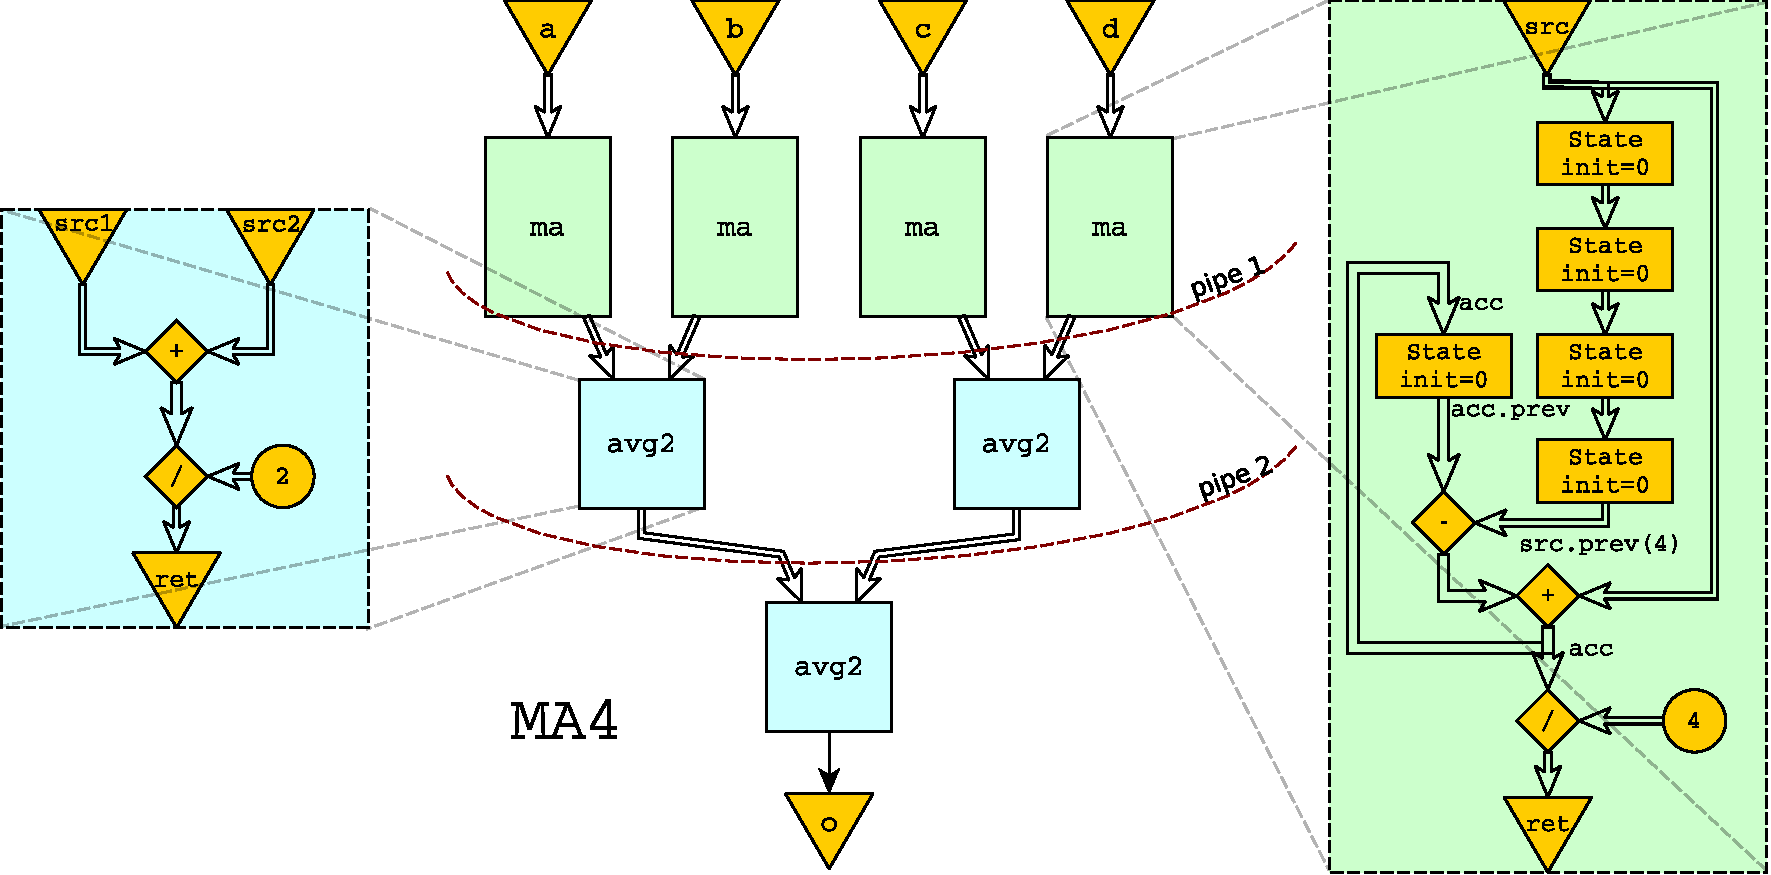
\includegraphics[width=0.92\linewidth]{graphics/ma.pdf}
  \captionsetup{justification=centering}
  \captionof{figure}{
  	The MA4 dataflow graph (the inputs are \code{a}, \code{b}, \code{c}, \code{d} and the output is \code{o}) \\ 
  	The entire design is a composition of the \code{ma} and \code{avg} functions (detailed blowouts are depicted as well). \\ 
  	The compiler places pipeline tags to achieve the required performance and the backend inserts registers accordingly. \\
  	The concurrent construction is implied from a sequential composition thanks to the dataflow abstraction. 
  }
\label{fig:MADraw}
\end{table*}

\section{The DFiant Language Overview}
\label{sec:dfiant}
DFiant is a Scala library and thus possesses various rich type safe language constructs. DFiant also incorporates unique language semantics that enable dataflow-based hardware description. Throughout this section we elaborate on these constructs and semantics via our running example, a four-by-four moving average (MA4) unit. The MA4 has four 16-bit integer input channels and is required to output the average of all channels, while each channel is averaged by a four-sample moving window continuously. The complete MA4 DFiant implementation and its equivalent dataflow graph are available in \fig{fig:MADFiant} and ~\ref{fig:MADraw}, respectively. \fig{fig:MAVHDL} presents a subset of the DFiant-generated VHDL (2008) code derived from lines 11-12 in \fig{fig:MADFiant}.


\subsection{Hello DFiant World!}
The MA4 DFiant code in \fig{fig:MADFiant} demonstrates the basics of any DFiant compilation program: it imports the \code{DFiant} library (line 1), creates the top-level design by extending the \code{DFDesign} library abstract class (lines 3-21), and creates a runnable application that instantiates the top design trait and compiles it into a VHDL file (line 32). 

The MA4 design is fairly straightforward. Lines 4-8 generate the signed dataflow ports and include a \code{0} value initialization (see Section~\ref{sec:state_constructs}). 
Lines 10-14 define the function \code{ma} that generates a single four-sample moving average, while lines 15-16 define the function \code{avg2} that generates a two-input average unit. Finally, lines 18-20 compose \code{avg2} and \code{ma} to generate the entire MA4 functionality and assign it to the output port \code{o}. We elaborate on the unique DFiant constructs and semantics in the next sections.


\subsection{Dataflow Semantics}
DFiant code is expressed in a sequential manner yet employs an asynchronous dataflow programming model to enable an intuitive concurrent hardware description. For this purpose, DFiant applies the following rules:

\subsubsection{Concurrency and Execution Order} 
Concurrency is implicit and the data scheduling order, or \textit{token-flow}, is set by the \textit{data dependency}. DFiant schedules all independent dataflow expressions concurrently, while dependent operations are synthesized into a guarded FIFO-styled pipeline. The MA4 dataflow graph in \fig{fig:MADraw} demonstrates the concurrent paths constructed from the dataflow dependency. 

\subsubsection{Basic Operations} 
\label{sec:basic_ops}
Each application of an arithmetic/logic operator is translated into the appropriate hardware construction and applies a dataflow \emph{join} on their arguments. The arguments require a valid token for consumption to produce a new token generated from the operations. For example, \code{+} in \code{avg2} joins \code{src1} and \code{src2} and requires a token from both to produce the token \code{src1 + src2}.

\subsubsection{Path Divergence} 
\label{sec:path_div}
Diverging paths are implicitly \emph{forked}, so token production is possible if all target nodes are ready to consume the token. For example, \code{acc} result in \code{ma} is forked into a division operation and the state feedback.	It is impossible to consume an invalid token and once a token is consumed it is invalidated.

\subsubsection{Constants} 
Any Scala primitive value is considered as a constant when applied as an argument to a dataflow operation. For example, the value \code{2} in \code{avg2} is a primitive \code{Int} and is considered a constant in the division operation. Semantically, a constant is an infinite token generator that produces a new token with the same initial value each time the token is consumed.

\subsubsection{Pruning}
Unused nodes always consume tokens and are discarded during compilation. 


\subsection{State Constructs and Semantics}
\label{sec:state_constructs}
In contrary to RTL languages, DFiant does not directly expose register and wire constructs. Instead, DFiant assumes every dataflow variable is a stream and provides constructs to initialize the token history via the \code{.init} construct, reuse tokens via the \code{.prev} construct, and update the state via the \code{:=} construct. Lines 11-12 in \fig{fig:MADFiant} along with their compiled VHDL representation in \fig{fig:MAVHDL} demonstrate the state semantics as follows:

\subsubsection{Initialization} The \code{.init} construct is accompanied by one or more token values and only sets the initial state history. For example, line 11 constructs a dataflow variable and initializes all of its history as zero value tokens. The history sequence written from left to right sets tokens from newest to oldest, respectively. If the sequence is accessed beyond the oldest token than the oldest token is repeatedly produced. If the history is empty (not initialized) then stall bubble tokens are produced when accessed (see \sect{sec:stall_bubbles}). It is also possible to directly place bubble tokens in the history by writing either $\phi$ or \code{Bubble}.  

\subsubsection{History Access} The \code{.prev} construct reuses the previous state token. The very first "reused" token is the one set via \code{.init}. It is also possible to call \code{.prev(step)} with a step number argument to reuse older stream values. For any dataflow value \code{a} and a given positive integer \code{step}, a call to \code{a.prev(step)} is equivalent to repeated $step$ applications of \code{a.prev.prev...prev}.
For example, in line 12 we reuse a \code{src} token from four steps ago. If the \code{src} token stream is "$1,2,3,4,...$" with a $0$ initialization, then the \code{src.prev(4)} token stream is "$0,0,0,0,1,2,3,...$".

\subsubsection{Distributive Property} The history access via \code{.prev} is distributive over all the basic DFiant operations. For example, the distributed \code{a.prev + b.prev} is equivalent to \code{(a + b).prev}. 
 
\subsubsection{Stall Bubbles} 
\label{sec:stall_bubbles}
Invoking \code{.prev} on an uninitialized dataflow variable generates a stall bubble. Stall bubbles are consumed and produced like any other token, yet a basic operation with a stall bubble token must produce a stall bubble token. Additionally, stall bubbles do not affect a feedback state. The backend compiler is responsible to generate the additional logic required for existing design stalls. 

\subsubsection{State Update Scheduling} The new updated token is pushed into a dataflow stream by using the \code{:=} assignment construct. There can be more then one assignment to same variable, however only the last assignment updates the state and occurs when all dependent dataflow firing rules are satisfied. This rule is similar to signal update semantics in VHDL processes.

\subsubsection{Default Self-Generation} 
\label{sec:default_self_gen}
Any dataflow \code{a} variable has an implicit self-assignment \code{a := a.prev} that comes immediately after the variable construction. This creates an equivalent reference between \code{a} and \code{a.prev} which leads to a more intuitive programming.
For example, in line 12 we used \code{acc - ...} and not \code{acc.prev - ...}, since both expressions are equivalent.

\vspace{2ex}

Another example that illustrates the benefits of the DFiant state constructs is a 32-bit Fibonacci series generator implementation provided in \fig{fig:FibGen}. The dataflow version is shorter than its VHDL counterpart~\cite{fibgenvhdl} and greatly resembles the formal Fibonacci definition: $F_0 = 0$, $F_1 = 1$, $F_n = F_{n-1} + F_{n-2}$ for $n > 1$. 

\begin{figure}[h]
  \centering
  \captionsetup{justification=centering}    

  \begin{minted}[xleftmargin=0.15\linewidth, xrightmargin=0.15\linewidth,frame=single,autogobble,linenos,tabsize=2,fontfamily=courier,fontsize=\fontsize{8}{9}\selectfont]{scala}
    trait FibGen extends DFDesign {
      val o = DFUInt[32] <> OUT
      val f = DFUInt[32] init (1, 0)
      f := f.prev + f.prev(2)
      o := f.prev(2) //output from 0
    }
  \end{minted}
  \captionof{figure}{A DFiant 32-bit Fibonacci series generator \\ Great resemblance to the formal Fibonacci definition}
  \label{fig:FibGen}
\end{figure}

Both \fig{fig:MAVHDL} and \fig{fig:FibGen} emphasize the advantages of DFiant state constructs over RTL registers and wires.
One advantage is that the DFiant code resembles its RTL counterparts, but is also very concise since state elements are automatically constructed when a stream history is accessed. Another advantage is portability, because state elements are not registers and therefore any type of state component is applicable. Our first synchronous backend indeed maps state elements to registers, but even an asynchronous backend can compile the same code and apply the Muller C-element~\cite{muller1957theory} as a state element. 

\subsection{Conditional Constructs and Semantics}
DFiant has \code{ifdf} and \code{matchdf} conditional constructs which logically resemble the Scala \code{if} and \code{match}, respectively. These dataflow conditional constructs are also very similar to their RTL counterparts and yield multiplexer hardware. However, their semantics follow the same dataflow \emph{join} and \emph{fork} rules we described in Sections \ref{sec:basic_ops} and \ref{sec:path_div}, and therefore all dataflow values used within the conditional constructs are joined together and all modified dataflow variables which are referenced outside the conditional constructs are forked as well. Of course, the default compiler yields a simple combinational structure if there is no need for this additional flow control logic.

\fig{fig:SeqDet} demonstrates a simple DFiant finite state-match (FSM) design that detects the sequence "1001". The VHDL~\cite{seqdetvhdl} implementation is very similar but is mainly longer because the split between the sequential and combination parts is automatically done by the DFiant compiler.
Note we did not need to directly refer to \code{state.prev} at line 7, thanks to the default self generation described in \sect{sec:default_self_gen}.

\begin{figure}[t]
  \centering
  \captionsetup{justification=centering}    
  
  \begin{minted}[xleftmargin=0.08\linewidth, xrightmargin=0.08\linewidth,frame=single,autogobble,linenos,tabsize=2,fontfamily=courier,fontsize=\fontsize{8}{9}\selectfont]{scala}
    trait SeqDet extends DFDesign {
      val seqIn  = DFBool() <> IN
      val detOut = DFBool() <> OUT
      object State extends Enum.Auto {
        val S0, S1, S10, S100, S1001 = Entry
      }
      val state = DFEnum(State) init State.S0
      matchdf(state)
      .casedf(State.S0) {
        detOut := 0
        ifdf (seqIn) {state := State.S1}
        .elsedf      {state := State.S0}
      }.casedf(State.S1) {
        detOut := 0
        ifdf (seqIn) {state := State.S1}
        .elsedf      {state := State.S10}
      }.casedf(State.S10) {
        detOut := 0
        ifdf (seqIn) {state := State.S1}
        .elsedf      {state := State.S100}
      }.casedf(State.S100) {
        detOut := 0
        ifdf (seqIn) {state := State.S1001}
        .elsedf      {state := State.S0}
      }.casedf(State.S1001) {
        detOut := 1
        ifdf (seqIn) {state := State.S1}
        .elsedf      {state := State.S10}
      }
    }
  \end{minted}
  \captionof{figure}{A DFiant "1001" sequence detector FSM \\ Very similar to its VHDL counterpart}
  \label{fig:SeqDet}
\end{figure}


%\subsection{Mutability}
%\label{sec:mutability}
%`:=` used to set update the state.
%DFiant supports dataflow variables mutability via the \code{:=} operator. Do not confuse with Scala-level mutability which is enabled by using \code{var} instead of \code{val}. Each dataflow class has two variations: an immutable class, which inherits from \code{DFAny\textbf{Val}} and a mutable class, which inherits from \code{DFAny\textbf{Var}} and accepts \code{:=}. The difference between the types enforces an immutable right-hand-side (RHS), where required, and a mutable variable creation. Consider, for instance, the DFiant implementation of \code{g} in Table \ref{tbl:StateExDefImpl}: \code{a} is immutable because it is a RHS addition between the dataflow variable \code{i} and a literal value \code{5}. Contrarily, \code{c} is mutable, since it is a dataflow variable constructor (\code{.init} constructs a new initialized variable, while preserving the mutability trait). 
%
%Fig.~\ref{fig:Inherit} demonstrates a dual class definition for every type  (immutable and mutable). The naming convention helps to reason about the mutability. For example, \code{DFBits} and \code{DFBits.Var} are immutable and mutable classes, respectively. Constructing a new variable via \code{DFBits} (e.g, \code{val a = DFBits[5]}) returns the mutable \code{DFBits.Var[5]}. Usually, we either receive or return an immutable type, hence we do not require annotating a type with its mutable variation. In cases where we want to return a mutable type, we annotate it as an output port (see Section~\ref{sec:io_ports}).
%
%DFiant's code safety is enforced by maintaining the 'DF-mutability' trait while aliasing (accepting the ':=' operator). This means that an alias of a \textbf{Var}, is still a \textbf{Var}, and can be assigned, while an alias of a \textbf{Val} cannot. This concept is illustrated in ???, and further explained in ???:


\subsection{Hierarchy and Connectivity}
So far, all examples demonstrated a single dataflow design without any hierarchies. The MA4 design managed to create structural encapsulations and composition via Scala definitions. Earlier, in \sect{sec:motivation}, we stressed the importance of any HDL to support hierarchies via constructs that describe components, ports and their connections. For this purpose DFiant has \code{<>} to both construct dataflow ports and create connections between them.
when applied between a dataflow variable constructor 

\begin{table*}[t!]
  \small
  \begin{minipage}[t][9cm][t]{0.343\linewidth}
    \centering
    \captionsetup{justification=centering}
    \begin{minted}[xleftmargin=1em,linenos,autogobble,tabsize=2,framesep=1pt,frame=single,fontfamily=courier,fontsize=\fontsize{7}{8}\selectfont]{scala}
      //All networks have the same interface
      trait Network extends DFDesign {
        val iT = DFSInt[16] <> IN  //Top
        val iB = DFSInt[16] <> IN  //Bottom
        val oT = DFSInt[16] <> OUT //Top
        val oB = DFSInt[16] <> OUT //Bottom
      }
      //State in Top Connection
      trait NWLeft extends Network {
        iT.prev <> oT //Connection
        oB := iB + 5  //Assignment
      }
      //State in Bottom Assignment
      trait NWRight extends Network {
        iT <> oT * 3  //Connection
        oB := iB.prev //Assignment
      }
      //Parent box includes two sibling boxes
      trait NWParent extends Network {
        iT init (5, 7) //Initializing history
        iB init (2, 6) //Initializing history
        val nwL = new NWLeft {}
        val nwL = new NWRight {}
        nwL.iT <> iT
        nwL.iB <> iB
        nwR.oT <> oT
        nwR.oB <> oB
      }
      //Direct connections between siblings
      trait NWParDirect extends NWParent {
        nwL.oT <> nwR.iT
        nwL.oB <> nwR.iB
      }
      //Cross connections between siblings
      trait NWParCross extends NWParent {
        nwL.oT <> nwR.iB
        nwL.oB <> nwR.iT
      }
    \end{minted}
    \vfill
    \captionof{figure}{Various network designs \\ Featuring hierarchies and inheritance }
    \label{fig:BoxTopCode}
  \end{minipage}%
  \hfill
  \begin{minipage}[t][12cm][b]{0.64\linewidth}
    \centering
    \captionsetup{justification=centering}
    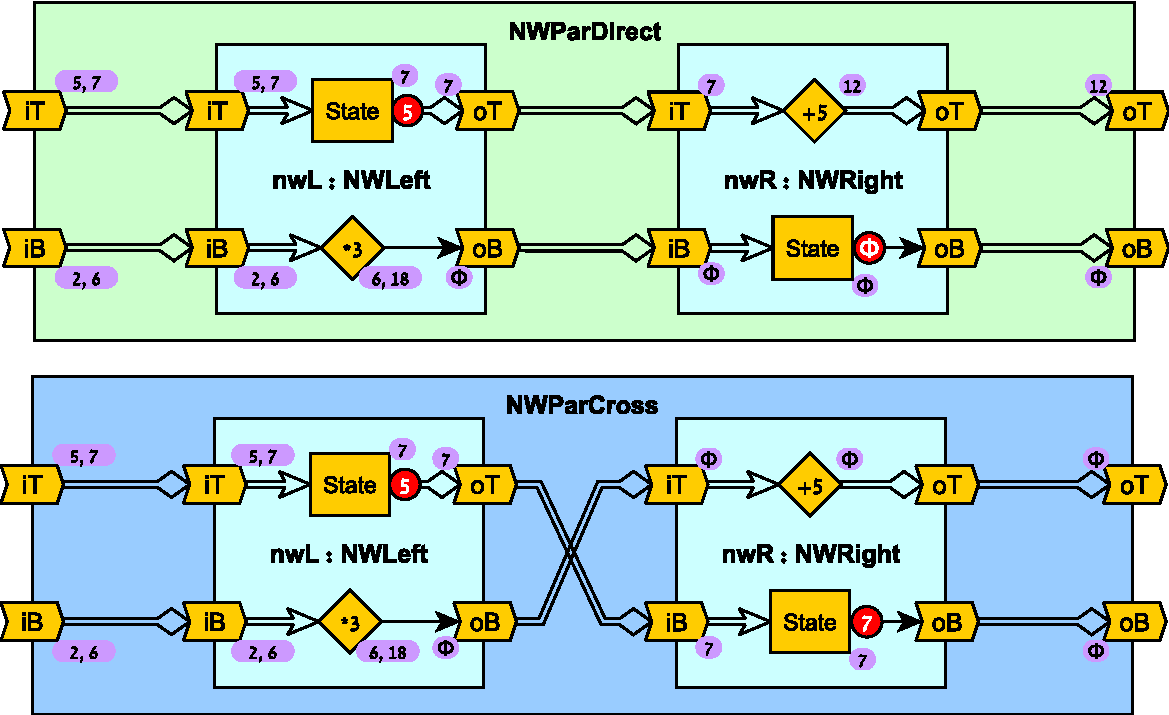
\includegraphics[width=0.9\linewidth]{graphics/connectivity.pdf}
    \captionof{figure}{
      Hierarichal drawing of \code{NWParDirect} and \code{NWParCross} \\
      The \colorbox{initcolor}{purple} numbers mark the initialization history as it is propagated according to the semantic rules of DFiant. The \colorbox{red}{\textcolor{white}{red}} numbers mark initial tokens generated by the state elements.
    }
    \vfill
    \label{fig:BoxTopDraw}
    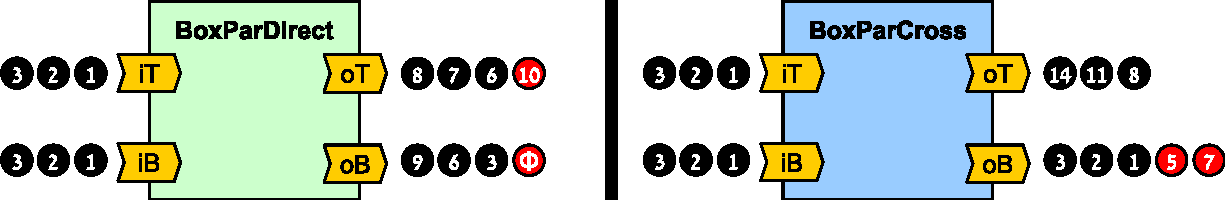
\includegraphics[width=0.9\linewidth]{graphics/connectivityTokens.pdf}
    \captionof{figure}{
      Input/Output token flow example to/from the two parent boxes (the rightmost tokens are the oldest). 
    }
    \label{fig:BoxTopTokens}
  \end{minipage}%
  \vspace{2ex}
  \hrule
  \vspace{2ex}
  \captionof{table}{Connection \code{<>} and Assignment \code{:=} Operator Comparison}
  \label{tbl:Box}
  \begin{tabular}{|c|c|c|}
    \hline 
    \textbf{Criteria} & \textbf{Connection \code{<>}} & \textbf{Assignment \code{:=}} \\ 
    \hline
    \begin{minipage}{0.1\textwidth}
      \flushleft
      Code
    \end{minipage} 
    &
    \begin{minipage}[c][1.5cm]{0.4\textwidth}
      \begin{minted}[autogobble,tabsize=2,framesep=1pt,fontfamily=pcr,fontsize=\fontsize{7}{8}\selectfont]{scala}
      trait IOConnection extends DFDesign {
        val i = DFUInt[8] <> IN
        val o = DFUInt[8] <> OUT
        o <> i
      }
      \end{minted}
    \end{minipage} 
    &  
    \begin{minipage}[c][1.5cm]{0.4\textwidth}
      \begin{minted}[autogobble,tabsize=2,framesep=1pt,fontfamily=pcr,fontsize=\fontsize{7}{8}\selectfont]{scala}
        trait IOAssignment extends DFDesign {
          val i = DFUInt[8] <> IN
          val o = DFUInt[8] <> OUT
          o := i
        }
      \end{minted}
    \end{minipage} 
    \\ 
    \hline 
    \begin{minipage}{0.1\textwidth}
      \flushleft
      Functional Diagram
    \end{minipage} 
    &
    \begin{minipage}[c][2cm]{0.10\textwidth}
      \centering
      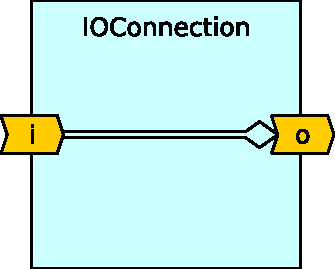
\includegraphics[height=1.8cm]{graphics/IOConnection.pdf}\\
    \end{minipage}%
    \hfill 
    \begin{minipage}[c][2cm]{0.27\textwidth}
      A double line arrow indicates a dataflow dependency \textbf{with} an initial condition dependency.
    \end{minipage} 
    &  
    \begin{minipage}[c][2cm]{0.10\textwidth}
      \centering
      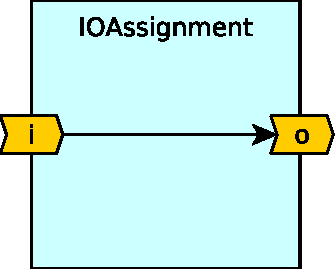
\includegraphics[height=1.8cm]{graphics/IOAssignment.pdf}\\
    \end{minipage}%
    \hfill 
    \begin{minipage}[c][2cm]{0.27\textwidth}
      A single line arrow indicates a dataflow dependency \textbf{without} affecting initial conditions of the consumer.
    \end{minipage} 
    \\ 
    \hline
    \begin{minipage}{0.1\textwidth}
      \flushleft
      Directionality \\and\\ Commutativity
    \end{minipage} 
    &
    \begin{minipage}[c][1.5cm]{0.42\textwidth}
      The operator is commutative, meaning \code{a <> b} is equivalent to \code{b <> a}. One argument is the \emph{producer}, while the other is the \emph{consumer}. The dataflow direction is sensitive to the context in which the operator is applied.
    \end{minipage} 
    &  
    \begin{minipage}[c][1.5cm]{0.42\textwidth}
      The operator is non-commutative, meaning \code{a := b} determines that \code{b} is the \emph{producer}, transferring data to the \emph{consumer} \code{a}.
    \end{minipage} 
    \\ 
    \hline
    \begin{minipage}{0.1\textwidth}
      Initialization
    \end{minipage} 
    &
    \begin{minipage}[c][1.2cm]{0.42\textwidth}
      Initialization is transferred to the consumer. If the consumer has both initialization via \code{.init} and connection, then the \code{.init} is the one that takes effect.
    \end{minipage} 
    &  
    \begin{minipage}[c][1.2cm]{0.42\textwidth}
      The consumer initialization is \textbf{not} affected.
    \end{minipage} 
    \\ 
    \hline
    \begin{minipage}{0.1\textwidth}
      \flushleft
      Mutation
    \end{minipage} 
    &
    \begin{minipage}[c][0.5cm]{0.42\textwidth}
      A consumer can only be connected once at each bit.
    \end{minipage} 
    &  
    \begin{minipage}[c][0.5cm]{0.42\textwidth}
      The same bit in a consumer can be assigned to 
    \end{minipage} 
    \\ 
    \hline
    \begin{minipage}{0.1\textwidth}
      \flushleft
      Statement Order
    \end{minipage} 
    &
    \begin{minipage}[c][0.8cm]{0.42\textwidth}
      Connections statements can be placed in any order. Connection from assigned variable TBD 
    \end{minipage} 
    &  
    \begin{minipage}[c][0.8cm]{0.42\textwidth}
      TBD.
    \end{minipage}% 
    \\ 
    \hline
  \end{tabular}% 
\end{table*}


%\subsection{IO Ports}
%\label{sec:io_ports}
%The class \textit{Box} from Table~\ref{tbl:Box} can also be coded as demonstrated in Fig.~\ref{fig:IOBox}. The annotation \code{DFVar $<>$ Dir} controls \textit{DFVar}'s access by encapsulating the variable with the dataflow port class, \code{DFPort}: an \code{IN} port can only be read (immutable), while an \code{OUT} port can only be modified (unreadable). DFiant has implicit conversions in place that selectively converts between \code{DFPort} and \code{DFAny} instances, without breaking mutability rules and type safety. The port annotations match the capabilities of traditional HDLs, and are noticeably absent from HLS languages such as C++. 

\subsection{Structural Composition and Generation}
DFiant expands traditional structural composition capabilities by utilizing Scala's object oriented features such as inheritance and polymorphism, as well as finite loops and recursive composition. The hierarchical compositions provide the scope and dependencies for the dataflow variables. The hierarchy itself is transparent to the dataflow graph, as if the entire design is flattened, inlined, and unrolled. Therefore, hierarchies in DFiant are synthesizable, highly reusable, and do not affect the design performance (may affect compilation time). 


\subsection{Bit-Accurate Operations and Type Inference}
DFiant supports various basic dataflow types such as \code{DFBool}, \code{DFBits}, \code{DFUInt}, and \code{DFSInt}.
All DFiant's dataflow types are bit-accurate and structurally static, with their bit-width set upon construction (e.g., \code{DFBits[5]} is a 5-bit vector). Operations between dataflow variables produce a bit-accurate result with the proper type inference. For example, an addition between an unsigned 5-bit variable (\code{DFUInt[5]}) and a signed 10-bit variable (\code{DFSInt[10]}) produces an adder that can be implicitly converted to a 10-bit signed variable, if carry is not required, or an 11-bit signed variable by explicitly invoking \code{.wc} from the addition. DFiant also allows operations between dataflow types and their corresponding Scala numeric types, by treating the Scala numeric types as constants (e.g., addition between \code{DFSInt} and \code{Int} variables). 


\subsection{Bit Aliasing and Casting}
Aliasing in DFiant enables referencing a part of a dataflow variable, by invoking \code{.bits(hiIdx, loIdx)}, which creates a bits vector alias that references the original variable at the given index parameters. Every change of a dataflow variable affects its alias and vice versa (similar to VHDL's signal aliasing). Since this function also casts the variable as \code{DFBits}, this feature is used as a raw-data cast between different dataflow types. Aliasing of an alias is also possible, while maintaining relative bits indexing. Aliasing preserves the mutability trait: an alias of an immutable variable is immutable, while an alias of a mutable variable is mutable. 


Fig.~\ref{fig:Aliasing} demonstrates aliasing code and its effect on the contents of a dataflow variable (\code{bits128}). Each line code does as follows:
\begin{enumerate}
  \item Constructs a new 128-bit vector, \code{bits128}, and clears it.
  \item Creates a new alias, \code{alias64}, which references the most significant 64 bits of \code{bits128}. Since \code{bits128} is a \code{DFBits} variable, there is no need to invoke \code{.bits()}, and we can apply the required indexes directly.
  \item Creates a new alias, \code{alias32}, which references the least significant 32 bits of \code{alias64}, which reference bits 64 to 95 of \code{bits128}.
  \item Constructs a new double precision floating point dataflow variable, \code{dbl}, and initialize its value as \code{1.0} (hexadecimal value of \code{0x3FF00...0}).
  \item Modifies the least significant byte of \code{dbl}.
  \item Sets the most significant bit of \code{bits128}.
  \item Assigns \code{dbl} to the least significant 64 bits of \code{bits128} through casting. All the bits of \code{dbl} are selected because \code{.bits()} is invoked without index parameters.
  \item Modifies a byte of \code{bits128}.
  
\end{enumerate}

\begin{figure}[h]
  \centering
  \begin{minipage}[b][3cm][b]{0.57\linewidth}
    \vfill
    \begin{minted}[xleftmargin=1.5em,linenos,autogobble,tabsize=2,framesep=1pt, frame=single,fontsize=\fontsize{8}{8}\selectfont]{scala}
      val bits128 = DFBits[128] := 0
      val alias64 = bits128(127, 64)
      val alias32 = alias64(31, 0)
      val dbl = DFDouble() := 1.0
      dbl.bits(7,0) := 0x28
      bits128(127) := 1
      bits128(63, 0) := dbl.bits()
      alias32(16, 8) := 0x57		    
    \end{minted}
    \vfill
    \subcaption{DFiant code}
  \end{minipage}%
  \hfill
  \begin{minipage}[b][3cm][b]{0.42\linewidth}
    \centering
    \vfill
		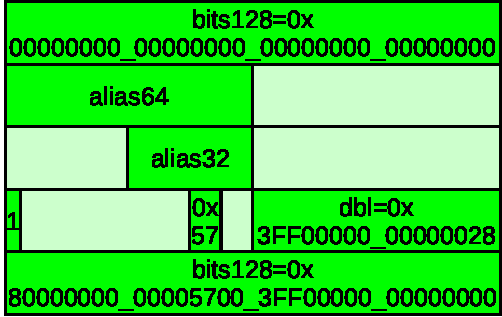
\includegraphics[width=\linewidth]{graphics/Aliasing.pdf} 
    \vfill
    \subcaption{Contents of \code{bits128}}
  \end{minipage}
  \captionof{figure}{Bit aliasing and casting example}
  \label{fig:Aliasing}
\end{figure}


\subsection{Simulation Constructs}
\label{sec:simulation}
Unlike VHDL and Verilog which were developed for simulation and only later were adapted for synthesis, DFiant was developed with focus on being a synthesizable language. Nonetheless, to test our designs we added some basic simulation-only constructs. To clearly separate pure simulation constructs from the rest of the language, we placed them under a separate name space -- \code{sim}. Additionally, all simulation constructs exist only within a simulation context. A simulation context is formed within a derivative of a dataflow design called \code{DFSimulation}. The \code{DFSimulation} construct is typically a toplevel instance that holds both our device-under-test (DUT) and the testing logic. Currently, the DFiant compiler only supports a handful of dedicated simulation constructs:
\code{sim.assert} to print errors if a condition is not satisfied; \code{sim.report} for printing messages; and finally \code{sim.finish} to finish the simulation. 
%All these constructs are very similar to their VHDL counterparts and in fact are



%+ C has no clear input/output notation. Input array and output array are the same.
%
%+ IDE: Intellisense, error highlighting, code completion, watches, println.
%+ Unified compilation
%+ Complete project build with the IDE. Compile results.
%Yes abstract away pipelining. No to scheduling control.
%
%Features we don't want
%simulations constructs.
%separate constraints file.
%
%VHDL Possible race conditions.
%
%
%+Include a summary table of RTL feature abstraction and how their are defined in DFiant.

